% 
% Interface
% @author Pieter Maene <pieter.maene@student.kuleuven.be>
%

\chapter{Kringverkiezing}
\label{chap:kringverkiezing}

Het Helios verkiezingssysteem werd in de praktijk gebruikt tijdens de kringverkiezing van de Vlaamse Technische Kring. Dit is de faculteitskring van de studenten burgerlijk ingenieur aan de KU Leuven. Om het systeem hiervoor te kunnen gebruiken, waren enkele aanpassingen nodig die overlopen worden in \ref{sec:kv:aanpassingen}. Gezien het cruciale karakter van een verkiezing, werd het systeem vervolgens uitgebreid getest (\ref{sec:kv:testen}). Tot slot wordt het verloop van de stemdag zelf besproken in \ref{sec:kv:stemdag}.

\section{Aanpassingen}
\label{sec:kv:aanpassingen}

\subsection{Shibboleth}

Shibboleth is het authenticatie mechanisme dat gebruikt wordt voor de centrale login van de KU Leuven. Iedere gebruiker kan uniek ge\"identificeerd worden aan de hand van zijn studentennummer. Alle stemgerechtigde kiezers voor een kringverkiezing hebben een dergelijke account. Helios had hier echter nog geen ondersteuning voor. Gezien het modulaire ontwerp van het authenticatiesysteem, was dit relatief eenvoudig toe te voegen.

%TODO Referentie naar Voter File in Helios

\npar De kieslijsten zelf werden opgemaakt door LOKO, de Leuvense studentenkoepel. Deze moesten we nog omgezet worden naar een bestand dat uitgelezen kon worden door Helios. Het studentennummer werd hierbij gebruikt als het unieke ID voor elke kiezer. Een probleem was hier wel dat de e-mailadressen van de kiezers niet mee opgenomen waren in deze lijsten. Deze kunnen wel opgenomen worden in het antwoord dat de server ontvangt nadat de student zich aangemeld heeft via de centrale login.

\subsection{Opkomst}

Bij VTK vertegenwoordigt het praesidium de studenten ook op onderwijsvlak. Om dit te kunnen doen, moet er volgens het reglement van LOKO een meerderheid behaald worden bij een opkomst van minstens 10\%.\cite{loko_kiesreglement_verkiezingen} De berekening van dit percentage werd dan ook toegevoegd zodat dit samen met de resultaten bekend gemaakt kon worden.

\subsection{Publicatie van het resultaat}

Helios publiceert het resultaat van de verkiezing standaard van zodra het bekend is. Het is echter traditie om deze pas om middernacht bekend te maken. Het systeem moest hier dus licht voor aangepast worden.

\section{Testen}
\label{sec:kv:testen}

Om er zeker van te zijn dat het systeem op de stemdag zelf goed zou functioneren, werd het na de installatie op de server getest. Hierbij werd niet alleen nagegaan of alles technisch in orde was, maar werd ook feedback gevraagd over de gebruiksvriendelijkheid. 

\subsection{Beheer}
\label{sec:kv:beheer}

%TODO Trustees

\npar Om het tellen van de stemmen te testen, werd een verkiezing aangemaakt met de echte vragen. Vervolgens werd aan de 60 leden van het huidige praesidium gevraagd om een stem uit te brengen.

\subsection{Stemhokje}
\label{sec:kv:stemhokje}

Tijdens het testen kwamen geen functionele problemen naar voor met het stemhokje. Toch kwam ook hier veel feedback op tijdens de test met het praesidium. Veel mensen vonden het stemmen niet intu\"itief. Er waren twee belangrijke bemerkingen. Ten eerste waren sommige bewoordingen te ingewikkeld. De interface is volledig in het Engels en er kwamen veel onbekende vaktermen in voor. Dit kon eenvoudig opgelost worden door iets eenvoudigere terminologie in de plaats te gebruiken.

\npar Ten tweede vonden velen het proces te ingewikkeld. Oorspronkelijk waren er vier stappen. Gebruikers kregen eerst een korte uitleg, gevolgd door het aanduiden van hun keuzes. Hierna konden deze gecontroleerd worden, waarna de stem ge\"encrypteerd werd. Daarna volgde nog een scherm (\ref{fig:kv:booth_submit}) waar gekozen kon worden om een audit te doen van de stem of ze te uploaden. In het laatste geval werd het stemhokje verlaten, maar moest de gebruiker nog eens bevestigen dat hij zijn stem wilde uitbrengen. Vooral deze twee laatste stappen vonden veel mensen verwarrend.

\begin{figure}
  \center{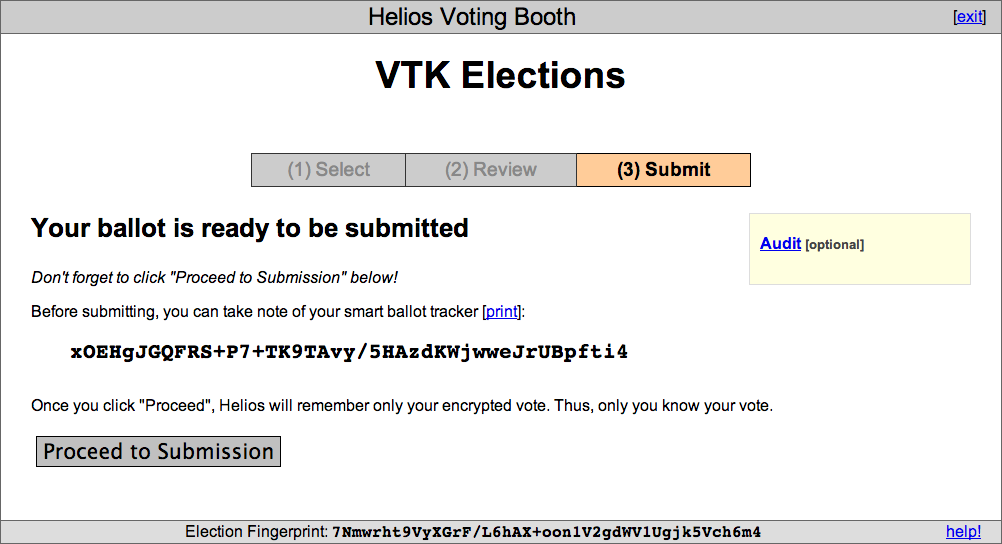
\includegraphics[width=\linewidth]{kv/booth_submit.png}}
  \caption{Laatste scherm van het stemhokje}
  \label{fig:kv:booth_submit}
\end{figure}

\npar Om dit proces te vereenvoudigen, werd de laatste stap van het stemhokje verwijderd. Na het bevestigen van zijn keuzes, wordt de kiezer onmiddellijk doorgestuurd naar het uploaden buiten het stemhokje. De audit van een stem werd verplaatst naar het scherm waar de keuzes bevestigd moet worden. Omdat de stem hiervoor reeds ge\"encrypteerd moet zijn, wordt dit nu gedaan na het beantwoorden van de laatste vraag. Het grootste nadeel hierbij is dat de encryptie opnieuw uitgevoerd moet worden wanneer de kiezer zijn stem wijzigt. In de huidige implementatie gaat dit echter al relatief vlot in moderne browsers. In de toekomst zal dit waarschijnlijk nog sneller kunnen door gebruik te maken van de Web Cryptography API (\ref{chap:web_cryptography_api}).

\subsection{Stresstest}

Er is elk jaar een opkomst van ongeveer 25\% bij de kringverkiezing van VTK, wat iets minder dan \np{1000} kiezers zijn. Daarom werd ook nagegaan of Helios ook een groot aantal stemmen nog correct kon verwerken. Hiervoor werd een aparte verkiezing aangemaakt met twee trustees en drie vragen. Vervolgens werden \np{1000} stemmen uitgebracht. Het resultaat kon van de eerste keer correct gedecrypteerd worden, dus hier was geen verdere actie nodig.

\npar Deze stemmen werden gegenereerd door een server-side actie. De kiezers stemmen normaal via het stemhokje, maar dat proces is moeilijk te automatiseren. Het grote verschil is dat de encryptie in Python in plaats van JavaScript gebeurt.

\section{Stemdag}
\label{sec:kv:stemdag}


